\documentclass[12pt]{book}

%These tell TeX which packages to use.
\usepackage{array,epsfig}
\usepackage{amsmath}
\usepackage{amsfonts}
\usepackage{amssymb}
\usepackage{amsxtra}
\usepackage{amsthm}
\usepackage{mathrsfs}
\usepackage{color}
\usepackage{eurosym}
\usepackage{times}
%Here I define some theorem styles and shortcut commands for symbols I use often
\theoremstyle{definition}
\newtheorem{defn}{Definition}
\newtheorem{thm}{Theorem}
\newtheorem{cor}{Corollary}
\newtheorem*{rmk}{Remark}
\newtheorem{lem}{Lemma}
\newtheorem*{joke}{Joke}
\newtheorem{ex}{Example}
\newtheorem*{soln}{Solution}
\newtheorem{prop}{Proposition}

\newcommand{\lra}{\longrightarrow}
\newcommand{\ra}{\rightarrow}
\newcommand{\surj}{\twoheadrightarrow}
\newcommand{\graph}{\mathrm{graph}}
\newcommand{\bb}[1]{\mathbb{#1}}
\newcommand{\Z}{\bb{Z}}
\newcommand{\Q}{\bb{Q}}
\newcommand{\R}{\bb{R}}
\newcommand{\C}{\bb{C}}
\newcommand{\N}{\bb{N}}
\newcommand{\M}{\mathbf{M}}
\newcommand{\m}{\mathbf{m}}
\newcommand{\MM}{\mathscr{M}}
\newcommand{\HH}{\mathscr{H}}
\newcommand{\Om}{\Omega}
\newcommand{\Ho}{\in\HH(\Om)}
\newcommand{\bd}{\partial}
\newcommand{\del}{\partial}
\newcommand{\bardel}{\overline\partial}
\newcommand{\textdf}[1]{\textbf{\textsf{#1}}\index{#1}}
\newcommand{\img}{\mathrm{omega}}
\newcommand{\ip}[2]{\left\langle{#1},{#2}\right\rangle}
\newcommand{\inter}[1]{\mathrm{int}{#1}}
\newcommand{\exter}[1]{\mathrm{ext}{#1}}
\newcommand{\cl}[1]{\mathrm{cl}{#1}}
\newcommand{\ds}{\displaystyle}
\newcommand{\vol}{\mathrm{vol}}
\newcommand{\cnt}{\mathrm{ct}}
\newcommand{\osc}{\mathrm{osc}}
\newcommand{\LL}{\mathbf{L}}
\newcommand{\UU}{\mathbf{U}}
\newcommand{\support}{\mathrm{support}}
\newcommand{\AND}{\;\wedge\;}
\newcommand{\OR}{\;\vee\;}
\newcommand{\Oset}{\varnothing}
\newcommand{\st}{\ni}
\newcommand{\wh}{\widehat}

%Pagination stuff.
\setlength{\topmargin}{-.3 in}
\setlength{\oddsidemargin}{0in}
\setlength{\evensidemargin}{0in}
\setlength{\textheight}{9.in}
\setlength{\textwidth}{6.5in}
\pagestyle{empty}

\begin{document}

\begin{center}
{\Large DATA 221 \\  Homework 3  (rev 2)}\\
\textbf{W. Trimble}\\ %You should put your name here
Due: Friday 2022-04-22 
\end{center}

\vspace{0.2 cm}

This question asks to you reproduce the graph of overfitting given in Hastie Elements of Statistical Learning Chapter 2.4.  The underlying source of the points in the graph was a lumpy mixture of isotropic (same variance in all directions) normal distributions.  We will have to generate the parameters of this distribution, generate samples from the distribution, and use k-nearest-neighbors to classify and overfit.

10 means for class 1 and 10 means for class 2 were drawn from a normal distribution in two dimensions centered at (0,1) and (1,0) and a standard deviation of (1,1) and no correlation between $x_1$ and $x_2$.   Points from each class are realized by choosing one of the subclusters randomly and drawing a random 2d normal with standard deviation 1/5 and no correlation.  This is now a lumpy distribution in two dimensions with 10 clusters for class 1 and 10 clusters for class 2.

\begin{enumerate}
\item
 Visualize the Bayes decision boundary between the two classes, the surfaces where the (true) density in class 1 equals the density in class 2.  Approximations are fine.
Plot a sample of 100 points from each class and present the sample as a scatter plot.  

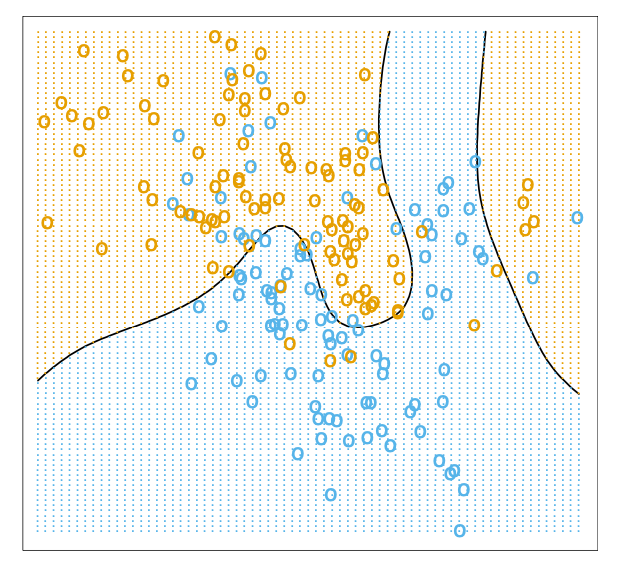
\includegraphics[width=3in]{hastie-bayesian.png}

\item
Perform K-nearest-neighbor classification for at least six values of $k$ ranging from 1 to 100; use the neighbors of each point to predict the class identity.  Evaluate accuracy as a function of $k$ for the training set (with 200 points).

\item
Generate a large sample of 10,000 points from each class.
Evaluate the accuracy of KNN classification (trained on the 200-point training set)  as a funciton of $k$ for the 20,000 points in the test set and plot the accuracy vs. $k$ for the training and the testing data on the same graph.    ( You could use these points, a sample from the distribution, to estimate the Bayes error rate using the probabilities from Q1, but you don't need to for full credit.)

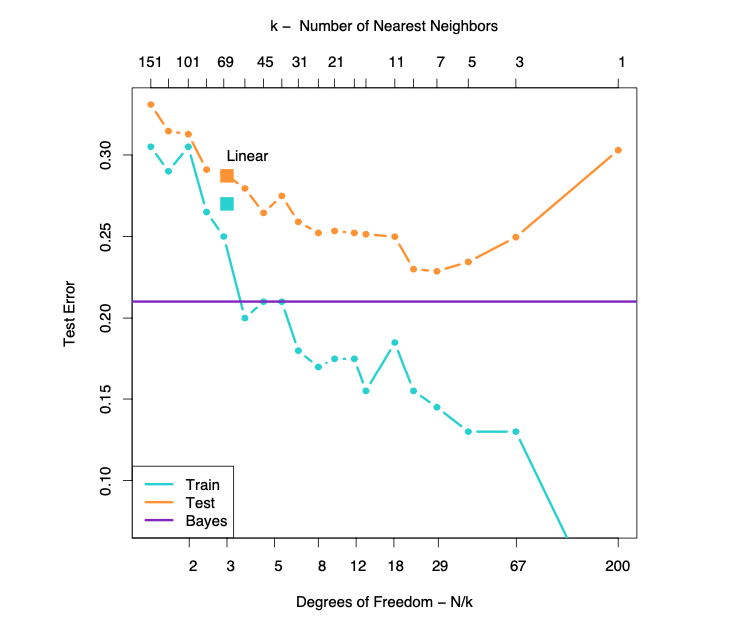
\includegraphics[width=4in]{hastie-generalization.png}

\item
Apply the same technique to the UCI "default of credit card clients Data Set" of 30,000 credit card customers in Taiwain in 2005. (Yeh \& Lien,  doi://10.1016/j.eswa.2007.12.020)   

Split the dataset 50/50 into training and test, and try to predict the \texttt{default.payment.next.month} using KNN classifiers for four different values of $k$.
Report accuracy on the testing and training datasets.

You have to choose how to measure distance in a vector space that includes indicator variables and payment amounts.  Try to choose something reasonable.

\texttt{https://archive.ics.uci.edu/ml/datasets/default+of+credit+card+clients}

\end{enumerate}
\end{document}


